\documentclass[journal,12pt,twocolumn]{IEEEtran}

\usepackage{setspace}
%\usepackage{gensymb}
\singlespacing
\usepackage[cmex10]{amsmath}

\usepackage{amsthm}

\usepackage{mathrsfs}
\usepackage{txfonts}
\usepackage{stfloats}
\usepackage{bm}
\usepackage{cite}
\usepackage{cases}
\usepackage{subfig}
\usepackage{float}
\usepackage{longtable}
\usepackage{multirow}

\usepackage{enumitem}
\usepackage{mathtools}
\usepackage{steinmetz}
\usepackage{tikz}
%\usepackage{circuitikz}
\usepackage{verbatim}
\usepackage{tfrupee}
\usepackage[breaklinks=true]{hyperref}
\usepackage{graphicx}
\usepackage{tkz-euclide}

\usetikzlibrary{calc,math}
\usetikzlibrary{automata, positioning}
\usepackage{listings}
    \usepackage{color}                                            %%
    \usepackage{array}                                            %%
    \usepackage{longtable}                                        %%
    \usepackage{calc}                                             %%
    \usepackage{multirow}                                         %%
    \usepackage{hhline}                                           %%
    \usepackage{ifthen}                                           %%
    \usepackage{lscape}     
\usepackage{multicol}
\usepackage{chngcntr}

\DeclareMathOperator*{\Res}{Res}

\renewcommand\thesection{\arabic{section}}
\renewcommand\thesubsection{\thesection.\arabic{subsection}}
\renewcommand\thesubsubsection{\thesubsection.\arabic{subsubsection}}

\renewcommand\thesectiondis{\arabic{section}}
\renewcommand\thesubsectiondis{\thesectiondis.\arabic{subsection}}
\renewcommand\thesubsubsectiondis{\thesubsectiondis.\arabic{subsubsection}}


\hyphenation{op-tical net-works semi-conduc-tor}
\def\inputGnumericTable{}                                 %%

\lstset{
%language=C,
frame=single, 
breaklines=true,
columns=fullflexible
}
\begin{document}


\newtheorem{theorem}{Theorem}[section]
\newtheorem{problem}{Problem}
\newtheorem{proposition}{Proposition}[section]
\newtheorem{lemma}{Lemma}[section]
\newtheorem{corollary}[theorem]{Corollary}
\newtheorem{example}{Example}[section]
\newtheorem{definition}[problem]{Definition}

\newcommand{\BEQA}{\begin{eqnarray}}
\newcommand{\EEQA}{\end{eqnarray}}
\newcommand{\define}{\stackrel{\triangle}{=}}
\bibliographystyle{IEEEtran}
\raggedbottom
\setlength{\parindent}{0pt}
\providecommand{\mbf}{\mathbf}
\providecommand{\pr}[1]{\ensuremath{\Pr\left(#1\right)}}
\providecommand{\qfunc}[1]{\ensuremath{Q\left(#1\right)}}
\providecommand{\sbrak}[1]{\ensuremath{{}\left[#1\right]}}
\providecommand{\lsbrak}[1]{\ensuremath{{}\left[#1\right.}}
\providecommand{\rsbrak}[1]{\ensuremath{{}\left.#1\right]}}
\providecommand{\brak}[1]{\ensuremath{\left(#1\right)}}
\providecommand{\lbrak}[1]{\ensuremath{\left(#1\right.}}
\providecommand{\rbrak}[1]{\ensuremath{\left.#1\right)}}
\providecommand{\cbrak}[1]{\ensuremath{\left\{#1\right\}}}
\providecommand{\lcbrak}[1]{\ensuremath{\left\{#1\right.}}
\providecommand{\rcbrak}[1]{\ensuremath{\left.#1\right\}}}
\theoremstyle{remark}
\newtheorem{rem}{Remark}
\newcommand{\sgn}{\mathop{\mathrm{sgn}}}
\providecommand{\abs}[1]{(\vert#1)\vert}
\providecommand{\res}[1]{\Res\displaylimits_{#1}} 
\providecommand{\norm}[1]{(\lVert#1)\rVert}
%\providecommand{\norm}[1]{\lVert#1\rVert}
\providecommand{\mtx}[1]{\mathbf{#1}}
\providecommand{\mean}[1]{E([ #1 )]}
\providecommand{\fourier}{\overset{\mathcal{F}}{ \rightleftharpoons}}
%\providecommand{\hilbert}{\overset{\mathcal{H}}{ \rightleftharpoons}}
\providecommand{\system}{\overset{\mathcal{H}}{ \longleftrightarrow}}
	%\newcommand{\solution}[2]{\textbf{Solution:}{#1}}
\newcommand{\solution}{\noindent \textbf{Solution: }}
\newcommand{\cosec}{\,\text{cosec}\,}
\providecommand{\dec}[2]{\ensuremath{\overset{#1}{\underset{#2}{\gtrless}}}}
\newcommand{\myvec}[1]{\ensuremath{\begin{pmatrix}#1\end{pmatrix}}}
\newcommand{\mydet}[1]{\ensuremath{\begin{vmatrix}#1\end{vmatrix}}}
\numberwithin{equation}{subsection}
\makeatletter
\@addtoreset{figure}{problem}
\makeatother
\let\StandardTheFigure\thefigure
\let\vec\mathbf
\renewcommand{\thefigure}{\theproblem}
\def\putbox#1#2#3{\makebox[0in][l]{\makebox[#1][l]{}\raisebox{\baselineskip}[0in][0in]{\raisebox{#2}[0in][0in]{#3}}}}
     \def\rightbox#1{\makebox[0in][r]{#1}}
     \def\centbox#1{\makebox[0in]{#1}}
     \def\topbox#1{\raisebox{-\baselineskip}[0in][0in]{#1}}
     \def\midbox#1{\raisebox{-0.5\baselineskip}[0in][0in]{#1}}
\vspace{3cm}
\title{Assignment 3}
\author{Taha Adeel Mohammed - CS20BTECH11052}
\maketitle
\newpage
\bigskip
\renewcommand{\thefigure}{\theenumi}
\renewcommand{\thetable}{\theenumi}
Download all python codes from 
\begin{lstlisting}
https://github.com/Taha-Adeel/AI1103/blob/main/Assignment_3/codes/assignment3.py
\end{lstlisting}
%
and latex-tikz codes from 
%
\begin{lstlisting}
https://github.com/Taha-Adeel/AI1103/tree/main/Assignment_3
\end{lstlisting}
\section{Problem (GATE 2008 (CS), Q.27)}
%%(GATE 2008 (CS), Q.27) \\
Aishwarya studies either computer science or mathematics everyday. If she studies computer science on a day, then the probability she studies mathematics the next day is 0.6. If she studies mathematics on a day, then the probability she studies computer science the next day is 0.4.
Given that Aishwarya studies computer science on Monday, what is the probablity she studies computer science on Wednesday?
\begin{enumerate}[label=(\Alph*)]
\begin{multicols}{2}
%\setlength\itemsep{2em}
\item 0.24
\item 0.36
\item 0.4
\item 0.6
\end{multicols}
\end{enumerate}
\section{Solution}
Let the random variables $X_i \in \{ 1,2 \}$ , $i=0,1,2, \cdots$ represent her studying CS(Computer Science) or mathematics respectively on the $i$th day. The transition matrix $P$ for the markov chain \{$X$\} (where $P_{ij}=\pr{X_t=j\, |\, X_{t-1}=i}$) is :-
\begin{align}
P=\begin{bmatrix}
x & 0.6 \\
0.4 & y 
\end{bmatrix}
\end{align}
\par As $X_i=0 \text{ and } X_i=1$ are mutually exclusive, we can easily calculate $x$ and $y$.
\begin{align}
   x=\pr{X_{i} = 0 \,|\, X_{i-1}=0} &= 1-\pr{X_{i} = 1 \,|\, X_{i-1}=0}\nonumber
    \\&= 0.4 \label{x}\\
    y=\pr{X_{i} = 1 \,|\, X_{i-1}=1} &= 1-\pr{X_{i} = 0 \,|\, X_{i-1}=1}\nonumber
    \\&= 0.6 \label{y}
\end{align}
\begin{figure}[h]
    \centering
     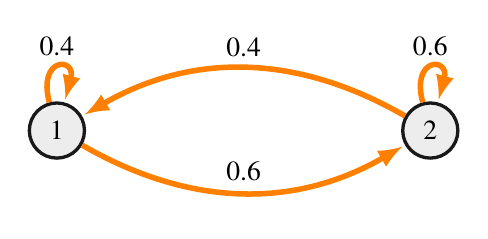
\begin{tikzpicture}[
roundnode/.style={circle, draw=black!90, fill=black!7, very thick, minimum size=7mm},
]
%Nodes
\node[roundnode]        (Computer_Science)        {1};
\node[roundnode]        (Mathematics)       [right=4cm of Computer_Science] {2};

%Lines
 \draw[every loop,
        auto=right,
        line width=0.7mm,
        >=latex,
        draw=orange,
        fill=orange]
            (Computer_Science) edge[bend right, auto=left]  node {0.6} (Mathematics)
            (Mathematics) edge[bend right, auto=right] node {0.4} (Computer_Science)
            (Computer_Science) edge[loop above]             node {0.4} (Computer_Science)
            (Mathematics) edge[loop above]             node {0.6} (Mathematics);
\end{tikzpicture}
    \par{Markov Diagram}

\end{figure}
\par The $\pr{X_{0+t}=i | X_{0}=j}$ is the $(i,j)$th position of $P^{\,t}$. Therefore $\pr{X_{2}=1 | X_{0}=1}$ is the $(1,1)$th position of $P^2$.
\begin{align}
    P^2=\begin{bmatrix}
0.4 & 0.6 \\
0.4 & 0.6
\end{bmatrix}\times
\begin{bmatrix}
0.4 & 0.6 \\
0.4 & 0.6 
\end{bmatrix}=
\begin{bmatrix}
0.4 & 0.6 \\
0.4 & 0.6 
\end{bmatrix}
\end{align}
\par $\therefore$ The probability she studies computer science on Wednesday is $P_{1\,1}^{\,2} = 0.4$.\\
(\textbf{Ans: Option (C)})
%%\begin{table}[h]
%%    \centering
%%    \begin{tabular}[width=\columnwidth]{|c|c|c|c|}
%%         \hline
%%        \textbf{Subject}&\textbf{X$_i$}&\textbf{$\pr{X_i | X_{i-1}=0}$} &\textbf{$\pr{X_i | X_{i-1}=1}$} \\
%%        \hline    
%%         CS&0&x (Ref \eqref{x})&0.4\\
%%         \hline
%%         Maths&1&0.6&y (Ref \eqref{y})\\
%%         \hline
%%    \end{tabular}
%%\end{table}
 
%%\begin{align}
%%    \therefore \pr{X_i=0}&=\pr{X_{i} = 0 \,|\, X_{i-1}=0}\times \pr{ X_{i-1}=0}\nonumber\\
%%    &+ \pr{X_{i} = 0 \,|\, X_{i-1}=1}\times \pr{ X_{i-1}=1}  \nonumber\\
%%    &=0.4\times\left( \pr{ X_{i-1}=0}+\pr{ X_{i-1}=1} \right) \nonumber\\
%%    &=0.4 \times 1 = 0.4
%%\end{align}
%Therefore, the probability that Aishwarya studies computer science on any day is $0.4$. So, the probability she studies computer science on Wednesday is also 0.4\\
% (\textbf{Ans: Option (C)})\\
%%\par Alternatively, the probability she studies CS on Wednesday($i=2$) can be found by($\because X_0=0$) :
%%\begin{align}
%%    \pr{X_2=0}&= \pr{X_1=0|X_0=0}\times \pr{X_2=0|X_1\hspace{-0.1cm}=\hspace{-0.1cm}0}\nonumber\\
%%    &+  \pr{X_1=1|X_0=0}\times \pr{X_2=0|X_1\hspace{-0.1cm}=1\hspace{-0.1cm}}\\
%%     &= 0.4\times 0.4 + 0.6\times0.4\\
%%     &=0.4
%% \end{align}
%%(\textbf{Ans: Option (C)})
\end{document}
